

\lecture{Álgebra Booleana: Introdução}{lec02}

\frame{\title{Álgebra Booleana e Aplicações}\titlepage}

\section{George Boole}

\begin{frame}{Boole}
  \framesubtitle{George Boole, 1815--1864}

   A Álgebra Booleana é um Sistema matemático apresentado por George
    Boole no livro ``An Investigation of the Laws of Thought'' em
    1854.

  \begin{columns}
    \begin{column}{.5\textwidth}
    \includegraphics[scale=.3]{\imgdir/lawsofthought.png}
    \end{column}
    
    \begin{column}{.5\textwidth}
      $$ x + y = x + (1-x)y$$
    \end{column}

  \end{columns}

\end{frame}

\begin{frame}{``Primeira'' aplicação}
  \framesubtitle{Claude Elwood Shannon, 1916--2001}
 
     Em 1938, Claude Shannon utilizou a algebra booleana para a
    solução de problemas de circuitos de telefonia com relés.
 
  \includegraphics[scale=.3]{\imgdir/shannon.png}
\end{frame}

\begin{frame}[fragile]{Comutação de relês}
  \def\dx{1cm}\def\dy{.5cm}
  \tikzset{every path/.style={draw},
    dot/.style={circle,inner sep=1pt,fill,label={#1},name=#1},
    dOt/.style={circle,inner sep=.75pt,anchor=east,label={#1},name=#1,draw}}

  \begin{tikzpicture}
    \path  (0,0) node[dot] {} -- (\dx,0);
    \path  (\dx,0) -- +(\dx/2,.5*\dy);
    \path (1.5*\dx,0) node[dOt=A] {} -- +(\dx,0) node[dot] {};
  \end{tikzpicture}\vspace{\dx}

  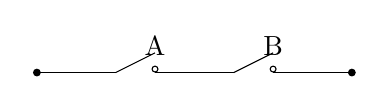
\begin{tikzpicture}
    \path (0,0) node[dot] {} -- (\dx,0);
    \path (\dx,0) -- +(\dx/2,.5*\dy);
    \path (1.5*\dx,0)  node[dOt=A,above] {} -- +(\dx,0);
    \path (2.5*\dx,0) -- +(\dx/2,.5*\dy);
    \path (3*\dx,0) node[dOt=B,above] {} -- +(\dx,0) node[dot] {};
  \end{tikzpicture}\vspace{\dx}

  \begin{tikzpicture}
    \path  (0,0) node[dot] {} -- (\dx,0);
    \foreach \y/\l in {1/A,-1/B} {
      \path (\dx,0) -- +(0,\y*\dy);
      \path (\dx,\y*\dy) -- +(.5*\dx,0);
      \path (1.5*\dx,\y*\dy) -- +(.5*\dx,.5*\dy);
      \path (2*\dx,\y*\dy)  node[dOt=\l,above] {} -- +(.5*\dx,0);
      \path (2.5*\dx,\y*\dy) -- +(0,-\y*\dy);
    }
    \path (2.5*\dx,0) -- +(\dx,0) node[dot] {};
  \end{tikzpicture}
\end{frame}

%%%%%%%%%%%%%%%%%%%%%%%%%%%%%%%% BUFFER

\ifnum1=2

\titleslide

\position{title}\Title
\position{by}{Apresentação}
\position{author}\Author
\position{date}\Date

\endtitleslide

\section{Início}

\slide[Ementa]

\Step[visible=true] Introdução: histórico, motivações, aplicações, notação moderna.

\Step[visible=true] {Teoria dos Conjuntos}.

\Step[visible=true] {Álgebras, expansões e expressões Booleanas}.

\Step[visible=true] Formas canônicas.

\Step[visible=true] Aplicações: 
$$\vbox{\small
     \item{$\star$} Circuitos lógicos combinacionais, aritmética digital,
       dispositivos de memória, análise de circuitos;
     \item{$\star$} Estrutura de dados: árvores de decisão binária;
     \item{$\star$} Algoritmos combinatórios.}
$$

\endslide

\slide[Método]

\Step[visible=true] Aulas expositivas: {\it slides\/}, lousa;

\Step[visible=true] Resolução de $\uparrow$ exercícios;

\Step[visible=true] eventualmente {Lógica Temporal de Ações}, programa para
     especificação de sistemas computacionais.

\endslide

\slide[Avaliação]

\Step[visible=true]   2 { Provas};

\Step[visible=true]   2 {Trabalhos};

\Step[visible=true]    eventualmente Lista de Exercícios.

\endslide

\slide[Livro-Texto]

   \Step[visible=true] cadê?

   \Step[visible=true] Notas de aulas.

\endslide

\bye

\fi

